\documentclass[conference]{IEEEtran}
\IEEEoverridecommandlockouts
% The preceding line is only needed to identify funding in the first footnote. If that is unneeded, please comment it out.
\usepackage{cite}
\usepackage{amsmath,amssymb,amsfonts}
\usepackage{algorithmic}
\usepackage{graphicx}
\usepackage{textcomp}
\usepackage{xcolor}

% Non Template Packages Star
\usepackage{placeins}
% Non Template Packages End

\def\BibTeX{{\rm B\kern-.05em{\sc i\kern-.025em b}\kern-.08em
    T\kern-.1667em\lower.7ex\hbox{E}\kern-.125emX}}
\begin{document}

\title{Almond Classification Using Neural Networks with Hybrid Learning\\
{\footnotesize \textsuperscript{*}COS 711 Assignment 2}
}

\author{\IEEEauthorblockN{1\textsuperscript{st} Damian Jordaan}
\IEEEauthorblockA{\textit{Department of Computer Science} \\
\textit{University of Pretoria}\\
Pretoria, South Africa \\
u20473509@tuks.co.za}
}

\maketitle

\begin{abstract}
This report presents a neural network-based approach to classifying almond types and compares different learning techniques. The dataset comprises 2803 samples with 12 distinct features derived from almond images. In this dataset, various futures have missing elements, and some calculated features are present. Various data preprocessing techniques were applied, including missing value imputation, feature transformation and feature scaling. We performed Hyperparameter optimization using Bayesian optimization and grid search. The model's performance is evaluated through the mean of its accuracy and f-score over multiple independent runs. Additionally, we compared traditional gradient-based training algorithms, such as resilient backpropagation (RProp), against other optimizers and implemented a hybrid learning approach that integrates gradient updates from multiple algorithms. Results demonstrated that hybrid learning did not perform better than the optimal optimizer for this problem.
\end{abstract}

\begin{IEEEkeywords}
Almond classification, Neural networks (NN), Hybrid learning, Hyperparameter optimization, Resilient backpropagation (RProp)
\end{IEEEkeywords}

\section{Introduction}
This report focuses on the problem of almond classification, which involves classifying almonds into one of three types—Mamra, Sanora, or Regular—based on numeric features extracted from images.

\subsection{Almond Dataset}

The dataset used in this study includes 2803 samples. Due to constraints in the imaging setup, some features have missing values that need to be processed. Additionally, some of the features are calculated from other features. This report will detail some of the different data preprocessing methods, discuss their performance, and attempt to find the method that should yield the best performance.

\subsection{Hyperparameter optimization}

Hyperparameter optimization is crucial to improving a model's predictive performance. This optimization process involves tuning parameters such as learning rate, batch size, and network architecture. We use the Bayesian optimization strategy to identify the best-performing configurations based on general parameter tuning and then further tune the parameters using a grid search strategy.

\subsection{Neural Network gradient-based optimizers and Hybrid Learning}

This study also explores hybrid learning techniques by integrating the strengths of multiple gradient-based optimizers, such as resilient backpropagation (RProp) and Nadam. By averaging the weight update value from different algorithms, hybrid learning aims to enhance convergence speed and stability, potentially leading to improved accuracy over conventional training methods. This report details the hyperparameter tuning for various optimizers and compares their performance for this problem. Apart from RProp, we select the best-performing optimizer to create a hybrid learning optimizer that averages the weight updates from RProp and the best-performing optimizer.

\subsection{Experiment Results and Model Performance}

The model's performance is measured using a combination of accuracy and f-score. It is then given a value that is the minimum of the two metrics.

 
\section{Background}

This study approaches the classification task using a supervised neural network model trained on a dataset of numeric features extracted from almond images. The dataset includes 2803 samples with 12 features per sample, capturing characteristics like length, width, and thickness. However, due to image orientation limitations, only two of these three primary dimensions are present for each sample, which complicates the classification process. Careful preprocessing is necessary to address these missing values and scale features appropriately for effective neural network training.

\subsection{Equations}

\begin{equation}
\text{Accuracy} = \frac{TP + TN}{TP + TN + FP + FN}
\end{equation}
\begin{equation}
\text{Precision} = \frac{TP}{TP + FP}
\end{equation}
\begin{equation}
\text{Recall} = \frac{TP}{TP + FN}
\end{equation}
\begin{equation}
F_1 = 2 \cdot \frac{\text{Precision} \cdot \text{Recall}}{\text{Precision} + \text{Recall}}
\end{equation}

 
\subsection{Hyperparameters}

General Hyperparameters

\begin{itemize}
    \item \textbf{test\_size}: Determines the proportion of the dataset reserved for testing the model's performance after training. Commonly expressed as a decimal (e.g., 0.2 for 20\% of data), this split helps evaluate the model's generalization ability on unseen data.
    \item \textbf{batch\_size}: Specifies the number of samples the model processes before updating the model's parameters. Smaller batch sizes allow for more frequent updates, potentially leading to faster convergence, while larger batch sizes provide more stable updates but may slow down learning.
    \item \textbf{epochs}: Defines the number of complete passes through the entire training dataset. Higher values allow the model more time to learn, but excessive epochs may lead to overfitting, where the model performs well on training data but poorly on test data.
    \item \textbf{patience}: Used in early stopping criteria to prevent overfitting. Patience is the number of epochs to wait after a performance improvement before stopping training. If the model's performance (e.g., validation loss) does not improve within the specified patience interval, training will stop early.
    \item \textbf{min\_delta}: Sets the minimum threshold for a performance improvement to be recognized during training. Changes smaller than min\_delta are considered negligible. This value works with patience to help determine when training should stop if progress stalls.
    \item \textbf{starting\_hidden\_layer\_size}: Specifies the number of neurons in the initial hidden layer. This value can influence the model's ability to capture complex patterns; too few neurons may limit learning, while too many can increase computational cost and risk of overfitting.
    \item \textbf{number\_hidden\_layers}: Indicates the total number of hidden layers in the neural network. Additional hidden layers enable the network to learn more complex representations and increase model complexity and computational requirements.
    \item \textbf{hidden\_layer\_activation}: The activation function is applied to the neurons in each hidden layer. Common options include ReLU, tanh, or sigmoid functions, each introducing non-linearity to help the network model complex patterns.
    \item \textbf{output\_activation}: The activation function applied to the output layer shapes the network's output format. For instance, a softmax function is often used for multi-class classification, while the sigmoid function is typically used for binary classification.
    \item \textbf{learning\_rate}: Controls the size of steps taken during parameter updates in training. A high learning rate can accelerate training but may lead to instability, while a low learning rate provides more precise updates but may slow down the learning process.
    \item \textbf{loss: }The loss function used by the network. Example are 
\end{itemize}
Other Optimizer-specific Parameters

\begin{itemize}
    \item \textbf{beta\_1}: A parameter used in adaptive optimizers like Adam that controls the exponential decay rate for the first moment (mean) estimate of gradients. It typically has a value close to 1 (e.g., 0.9) and helps stabilize updates by balancing the influence of past gradients on current learning.
    \item \textbf{beta\_2}: Another parameter in optimizers like Adam, it controls the exponential decay rate for the second moment (variance) estimate of gradients. Typically set close to 1 (e.g., 0.999), it helps manage noisy updates, especially in the presence of sparse gradients.
    \item \textbf{epsilon}: A small constant added to the denominator in optimization algorithms (e.g., Adam, RMSprop) to prevent division by zero. It ensures numerical stability during weight updates, particularly when gradient values are very small.
    \item \textbf{initial\_step\_size}: In gradient-based optimizers, this parameter defines the initial size of each update step. It acts as a starting point for step size adjustments, balancing early progress with the potential need for later fine-tuning.
    \item \textbf{increment\_factor}: Used in algorithms that adjust step sizes dynamically, such as resilient backpropagation (RProp). When the gradient's direction remains consistent, this factor increases the step size, allowing the model to converge faster when progress is steady.
    \item \textbf{decrement\_factor}: Also used in step size-adjustment algorithms, it reduces the step size when the gradient's direction changes (indicating possible oscillation). This helps the model avoid overshooting and promotes smoother convergence.
    \item \textbf{min\_step\_size}: Sets the minimum allowable step size in adaptive optimizers. By capping the smallest steps, it prevents the model from becoming too slow to learn, even if the gradient becomes very small.
    \item \textbf{max\_step\_size}: Defines the upper limit for step sizes in algorithms with adaptive step adjustments. This cap prevents overly large updates that could destabilize learning, especially if gradients are unexpectedly high.
\end{itemize}

\subsection{Data Exploration Analysis}

\begin{table}[h]
    \centering
    \begin{tabular}{lrrrr}
        \hline
        Type            & MAMRA & REGULAR & SANORA & Total \\
        \hline
        Measure Format  &       &         &        &       \\
        LxD             & 306   & 316     & 320    & 942   \\
        LxW             & 359   & 325     & 320    & 1004  \\
        WxD             & 268   & 286     & 303    & 857   \\
        Total           & 933   & 927     & 943    & 2803  \\
        \hline
    \end{tabular}
    \caption{Number of entries per type and measurement format}
    \label{tab:DataBalance1}
\end{table}

The data in the almond classification data set is evenly split between the three types of almonds. Additionally, it is evenly split between the different measurement formats per almond type. ``tab.~\ref{tab:DataBalance1}'' This being the case, unbalanced classes are not a concern and are, therefore, not accounted for. 

\subsection{Optimizers}

\begin{itemize}
    \item \textbf{RProp (Resilient Backpropagation) Definition}: RProp, or Resilient Backpropagation, is a gradient-based optimization algorithm that adjusts the step size based solely on the direction of the gradient rather than its magnitude. By only considering the sign of the gradient, RProp aims to avoid the problems of vanishing or exploding gradients, making it suitable for networks with oscillatory or unstable learning. It adapts step sizes dynamically: increasing them when gradients consistently point in the same direction and decreasing them when the gradient direction changes.
    \item \textbf{Adam (Adaptive Moment Estimation) Definition}: Adam is a widely used adaptive optimization algorithm that combines ideas from both Momentum and RMSProp. It maintains running averages of both the gradient (first moment) and the squared gradient (second moment) to adapt the learning rate for each parameter individually. This approach enables faster convergence by adjusting step sizes based on both the recent gradient history and its variance, which helps stabilize updates and improve performance in sparse or noisy data settings.
    \item \textbf{Nadam (Nesterov-accelerated Adaptive Moment Estimation) Definition}: Nadam extends Adam by incorporating Nesterov momentum, which applies a correction step that "looks ahead" before updating the parameters. This foresight helps to reduce oscillations, especially in the early stages of training. Nadam retains the benefits of Adam's adaptive learning rates and momentum while improving convergence speed, making it especially effective for models that benefit from accelerated gradients and adaptive learning adjustments.
    \item \textbf{Other Optimizers:} Tensorflow's built-in classes were used by all other optimizers.
\end{itemize}

\section{Experiment Setup}

\subsection{General Information}

\begin{itemize}
    \item Epochs for all tests are set at 200 unless specified otherwise. 
    \item The test size for all tests is set at 20\% unless specified otherwise.
    \item Custom implementation of Nadam optimizer was ported/based on the Tensorflow implementation \cite{b3}.
\end{itemize}


\subsection{Data Preprocessing Variations}

For this experiment, three different data preprocessing methods were tested. Additionally, all calculated features were removed. Moreover, all features were normalized - except for length, width, and depth, which were instead min-max normalized to be within '0 and 1.' Furthermore, the length, width, and depth features are processed as one large feature when it came to applying normalization. In other words, they share a minimum and maximum value, as well as a mean and standard deviation value.

\begin{itemize}
    \item Method 1: In this method, the length, width, and depth were combined into length A and length B. Additionally, three columns are added - L, D, and W. In these columns, a '1' will be used where the original columns were present and a '0' will be used if no data was present in the original column. 
    \item Method 2: Same as method 1, except instead of adding 'L, D, and W' columns, one-hot encoding was used to represent the original columns. For example, if length and width were present, the representation would be 'L x W'
    \item Method 3: In this method, a '-1' was added wherever there were missing values in the length, width, and depth columns. 
\end{itemize}

\subsubsection{Other Missing Values}

Aspect Ratio and Eccentricity both have 64.18\% of data missing. Therefore these features are removed. They are also calculated making them less useful even if they can sometimes contain some useful information. The Roundness feature is also removed as there is not a very meningful data imputation method for this feature.

\subsection{Neural Network Basic Architecture}

For this experiment, a pyramid structure was used for the neural network, where an initial number of hidden layer neurons, as well as hidden layers were defined. The program rule then calculates the number of neurons in the subsequent hidden layers based on the number of hidden layers, such that the number of neurons in each hidden layer decreases evenly until the number of output neurons is reached. 

A pyramid structure for a neural network has been shown to have good generalized performance. \cite{b1}

\subsection{Early Stopping Mechanism}

For this project, an early stopping mechanism is implemented. This mechanism will stop the training of a neural network early if the change in accuracy is below a minimum over a certain number of epochs. The parameters are patience (determines the maximum number of epochs without meeting the minimum threshold) and min\_delta (the amount of change needed in the epochs). Patience is set to 10, and min\_delta is set to 0.01 for all experiments. Additionally, at the end of training, this mechanism will restore the model weights with the highest validation accuracy. This is done to avoid cases where the model would heavily overfit.

\subsection{Exploration Testing Setup Data}

This outlines the testing methodology for the three variations of data preprocessing. The three methods were tested on the basic pyramid neural network structure with a starting hidden layer size of '64-128', a test size of '0.2', and a batch size of '32' over 200 epochs. Thirty independent tests were conducted for each method. Additionally, the "Adam" optimizer was used.

\subsection{Exploration Testing Setup General Hyperparameters}

For this experiment, all globally applicable hyperparameters, excluding epoch, were tuned using Bayesian optimization. This was done over 500 test cases.
Parameters Tuned: optimizer ('adam', 'sgd', 'rmsprop' ), loss function ('categorical\_crossentropy', 'binary\_crossentropy', 'mean\_squared\_error' ), output\_activation ('softmax', 'sigmoid'), hidden\_activation ('relu', 'tanh', 'sigmoid'), learning\_rate, batch\_size (6-32), starting\_hidden\_layer\_size (16-128), number\_hidden\_layers (1-6)

\subsection{Exploration Testing Setup RProp}

In this test, only RProp's own hyperparameters were tuned: initial step size, increment factor, decrement factor, max step size, and min step size. The parameters were also tuned using Bayesian optimization over 500 test cases. 

\subsection{Exploration Testing Setup Optimizers}

In this test, a variety of different optimizers were tested, each with their own hyperparameters being tuned individually. The optimizers that were tested are "adam", "sgd", "rmsprop", "adamax", "adagrad", "adadelta", "nadam", "ftrl", "adamw", "adfactor"

\subsection{Final Data Preprocessing}

Based on the results of the exploration testing, a modification was made to the data preprocessing whereby the measurement features were processed using standard deviation instead of min-max. The reason for doing this was to allow for more identity in the data, as processing with min-max can lead to the loss of identity in the data.

\subsection{Final Testing Setup}

Based on the results of the exploration testing, the best optimizer was found to be "Nadam." As such, the hybrid optimization method is chosen to be a combination of RProp and Nadam. This is implemented as follows: First, the RProp weight update is calculated, then the Nadam weight update is calculated, then a weighted average is calculated for the two variables, and that weighted average is then applied to the weight of the neurones. 

The hybrid optimization, in addition to RProp and Nadam, were all tested with the best-performing hyperparameters from the exploration testing. Additionally, a grid search was performed for each using the hyperparameters batch size and hidden layer activation function. The batch size was tested for 3 possible sizes: 8, 32, and 64. 

\newpage

\section{Research Results }

\subsection{Exploration Testing Results Data Preprocessing Methods}

\begin{figure}[htbp]
\centerline{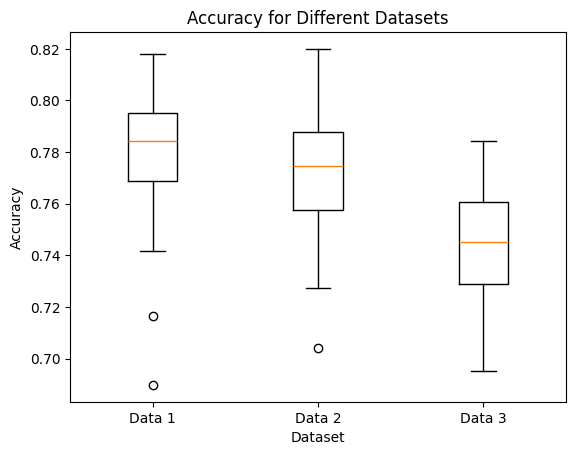
\includegraphics[width=0.9\columnwidth]{Ex Per Data Pre Pros Box Acc.png}}
\caption{The Accuracy Box plot for the different data preprocessing methodologies.}
\label{fig:Ex Per Data Pre Pros Box Acc}
\end{figure}

\FloatBarrier

\begin{figure}[htbp]
\centerline{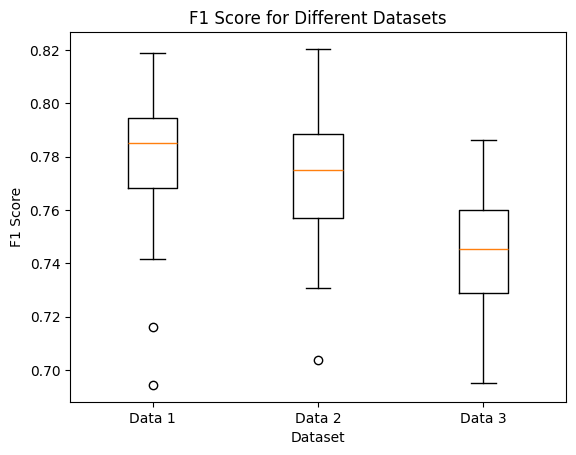
\includegraphics[width=0.9\columnwidth]{Ex Per Data Pre Pros Box F1.png}}
\caption{The F-score Box plot for the different data preprocessing methodologies.}
\label{fig:Ex Per Data Pre Pros Box F1}
\end{figure}

\FloatBarrier

(Data 1: method 1, Data 2: method 2, Data 3: method 3)

As shown in ``Fig.~\ref{fig:Ex Per Data Pre Pros Box F1}, ~\ref{fig:Ex Per Data Pre Pros Box Acc}'', methods 1 and 2 did better by a fairly large margin than method 3. This is unexpected because method 3, having '-1' in missing values, would balance out the other columns being limited to between '0 and 1.' Method 1 does the best overall - this is likely because it has 2 values in the identifier columns that perfectly balance out the 2 length columns. 

\newpage

\subsection{Exploration Testing Results General Hyperparameters}

Refer to Notebook for more data plots.\cite{b2}

\begin{figure}[htbp]
\centerline{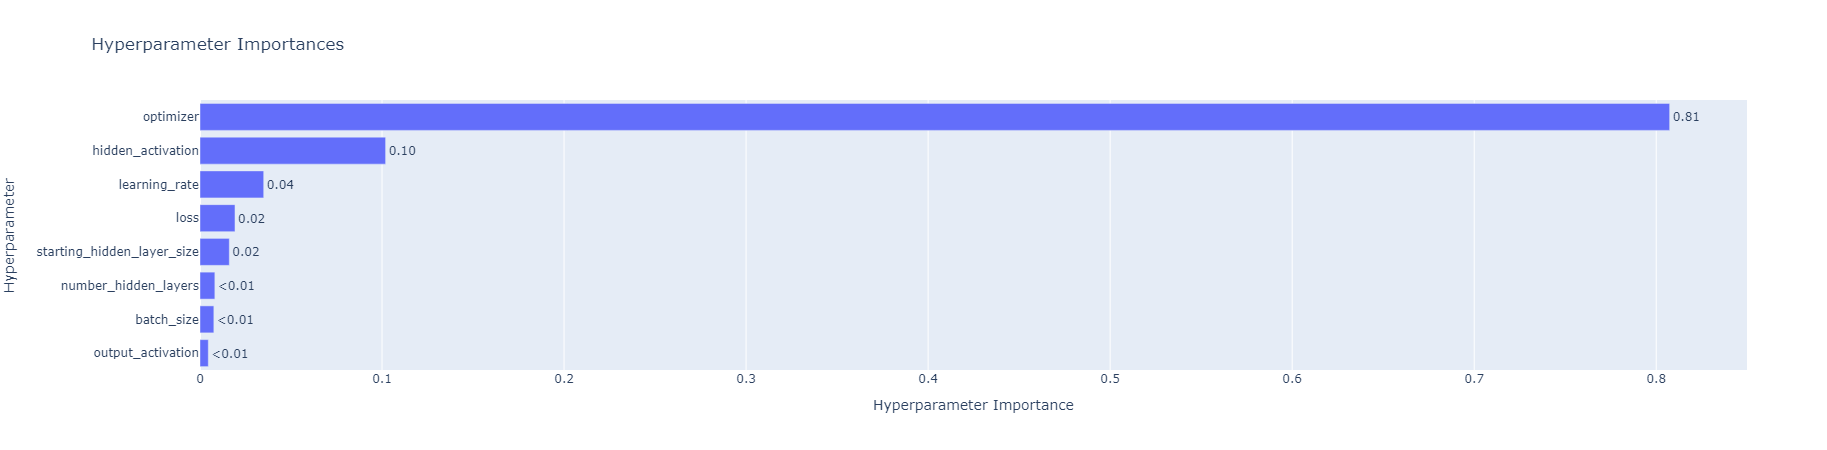
\includegraphics[width=\columnwidth]{Ex Gen Hyp Opt Res Imp.png}}
\caption{Test Parameter Importance.}
\label{fig:Ex Gen Hyp Opt Res Imp}
\end{figure}

\FloatBarrier

\begin{table}[h]
    \centering
    \begin{tabular}{|r|c|c|}
        \hline
        Parameter& Value &Importance\\ \hline
        Batch\_size& 8 &0.008\\ \hline
        starting\_hidden\_layer\_size& 123&0.02\\ \hline
        number\_hidden\_layers& 5&0.008\\ \hline
        loss function&           categorical\_crossentropy&0.02\\ \hline
 output\_activation& sigmiod&0.004\\\hline
 hidden\_activation& tanh&0.1\\\hline
 optimizer& adam&0.81\\\hline
 learning\_rate& 4.1627e-4&0.04\\\hline
    \end{tabular}
    \caption{Exploration General Hyperparameter Tuning}
    \label{tab:ExGenHyperTuning}
\end{table}

\FloatBarrier

The optimizer and hidden activation function have the highest importance. This is because the optimizer used completely determines how well the model is trained and, as such, how well it would perform. Additionally, the hidden layer activation function is of high importance because this will determine how well the model generalizes with a specific training algorithm.

The number of hidden layers and the size of the hidden layers have little effect on the model. While there is an increase in performance, increasing these values is negligible, and therefore, to make the model smaller, a hidden layer starting size of 64 and a number of hidden layers of 4 will be used for all subsequent models. 

Batch size has some effect on the model because it has an effect on the loss value. i.e. impacts training dynamics and loss values. Larger batch sizes can lead to larger loss values, which can mean that during training, the model oscillates more and it takes more epochs to reach lower loss values.

The output activation function had almost no effect between the different functions ('softmax', 'sigmoid'). As such, for all subsequent models and tests, softmax was chosen to be used as it would provide a probability distribution over the three classes.

The learning rate would have to be re-tuned as it is an optimizer-specific hyperparameter.

\subsection{Exploration Testing Results RProp}

\begin{figure}[htbp]
\centerline{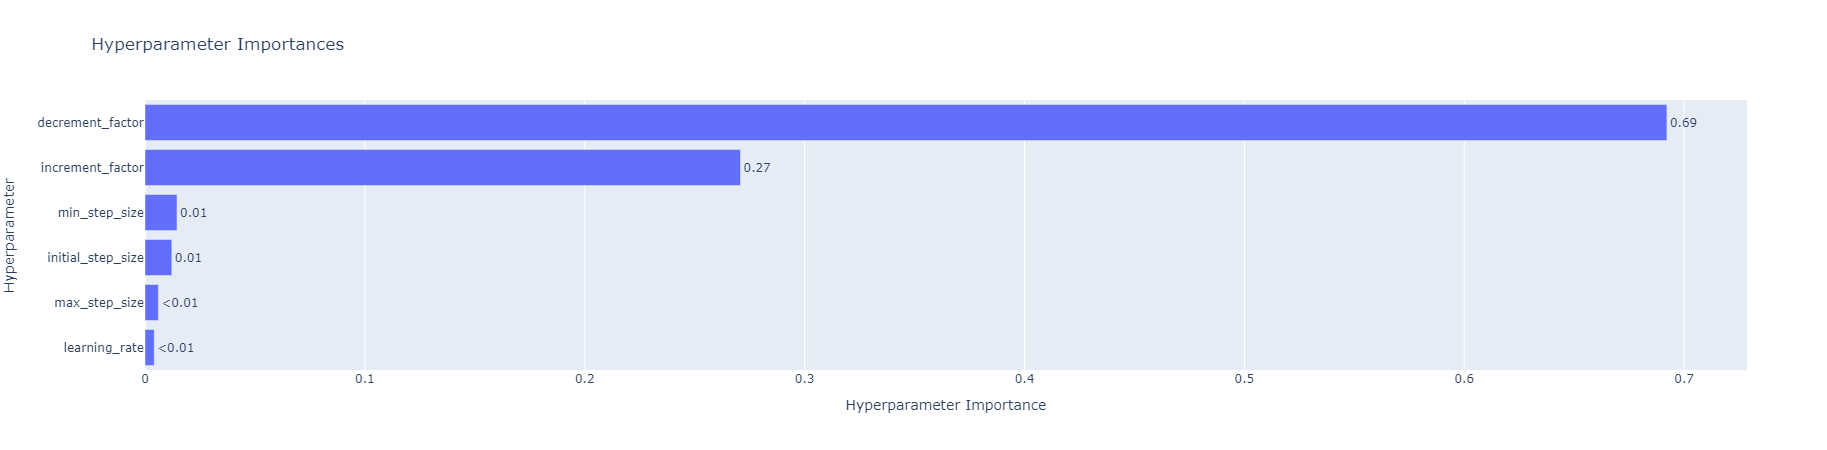
\includegraphics[width=\columnwidth]{Ex RProp Hyp Opt Res Imp.png}}
\caption{Test Parameter Importance.}
\label{fig:Ex RProp Hyp Opt Res Imp}
\end{figure}

\FloatBarrier

\begin{table}[htbp]
    \centering
    \begin{tabular}{|r|c|}\hline
 Parameter&Importance\\\hline
        \hline
        initial\_step\_size&0.01\\ \hline
        increment\_factor&0.27\\ \hline
        decrement\_factor&0.69\\ \hline
         min\_step\_size&0.01\\ \hline
        max\_step\_size&0.01\\ \hline
        learning\_rate&0\\\hline
    \end{tabular}
    \caption{RProp Experimental Parameter Importance}
    \label{tab:ExRPropParamImportance}
\end{table}

\FloatBarrier

For RProp, increment and decrement factors are of the highest importance. ``Fig.~\ref{fig:Ex RProp Hyp Opt Res Imp}'' This makes sense because these two determine the training algorithm's oscillation. 
Learning rate has no influence as it is not used by the RProp algorithm.

\subsection{Exploration Testing Results Optimizers}

\begin{figure}[htbp]
\centerline{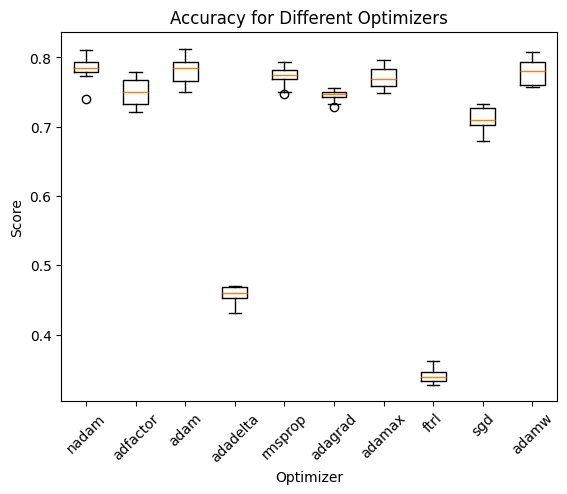
\includegraphics[width=\columnwidth]{Ex Optis Hyp Opt Res Box Acc.png}}
\caption{Box Plot for Diff. Optimizer performance.}
\label{fig:Ex Optis Hyp Opt Res Box Acc}
\end{figure}

% \newpage
\FloatBarrier

Nadam, Adam and Adamw seem to perform the best after tuning. Adadelta and ftrl perform the worst. The other optimizers are close in performance to the best three.
Nadam has the best overall performance, but only by a small margin. ``Fig.~\ref{fig:Ex Optis Hyp Opt Res Box Acc}''

Nadam, Adam, and AdamW use adaptive learning rates, which adjust the learning rate for each parameter based on the first and second moments of the gradients. This allows them to perform well, especially on this problem.

Adadelta uses adaptive learning rates, but it seems it is too aggressive or too conservative in its adjustments, leading to bad performance. FTRL (Follow-the-Regularized-Leader) is designed for sparse data and does not generalize well to this problem space.

Since there is less exploration of the learning rate due to the number of hyperparameters in this test, Adadelta and FTRL's sensitivity to hyperparameter settings \cite{b5} explain their bad performance. On the other hand Nadam, Adam, and AdamW are generally more robust to hyperparameter settings. \cite{b4} 

\subsection{Final Testing Results RProp}

\begin{figure}[htbp]
\centerline{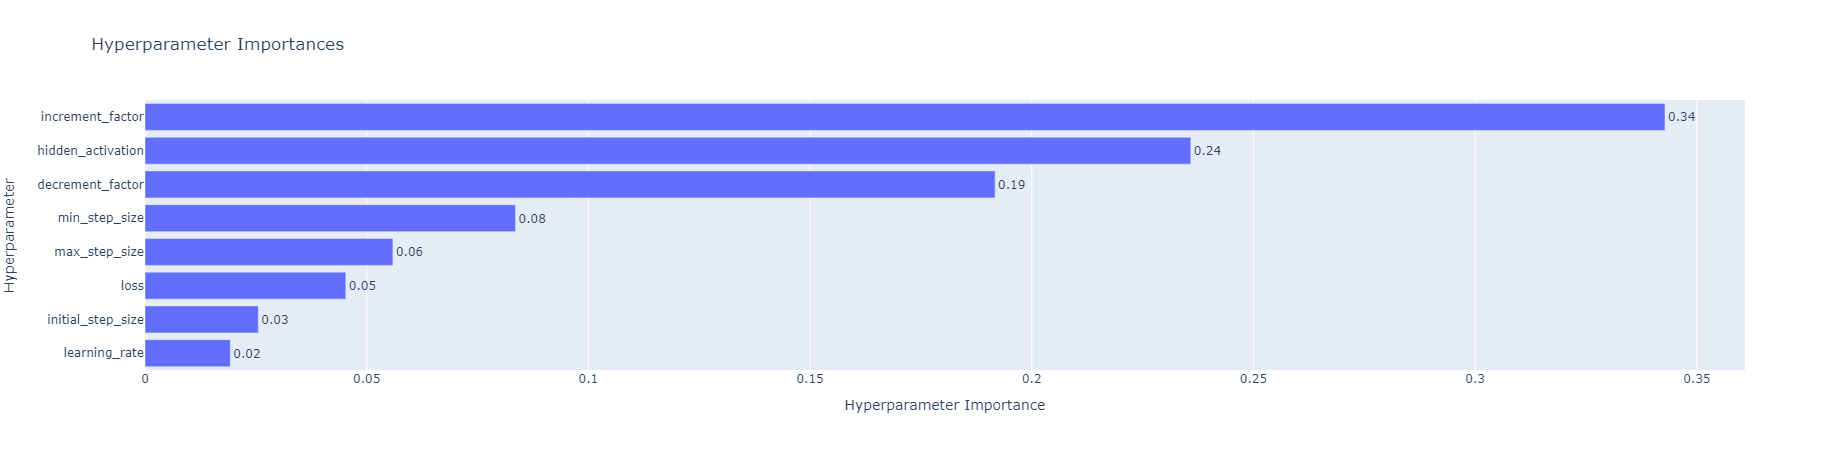
\includegraphics[width=\columnwidth]{F RProp Hyp Opt Res Imp.png}}
\caption{RProp parameter Importance}
\label{fig:F RProp Hyp Opt Res Imp}
\end{figure}

\FloatBarrier

\begin{table}[htbp]
    \centering
    \begin{tabular}{|r|c|c|}\hline
 Parameter& Tuned Value&Importance\\\hline
        \hline
        hidden\_activation& tanh&0.24\\ \hline
        initial\_step\_size& 0.0010&0.03\\ \hline
        increment\_factor& 1.1141&0.34\\ \hline
        decrement\_factor& 0.3694&0.19\\ \hline
         min\_step\_size& 0.0006&0.08\\ \hline
        max\_step\_size& 68.2485&0.06\\ \hline
        loss function & mean\_squared\_error&0.03\\\hline
    \end{tabular}
    \caption{RProp Parameter Tuning Result}
    \label{tab:RPropFinalParams}
\end{table}

\FloatBarrier

Similar results were obtained as with the initial experimentation. The change in importance could be due to the semi-random nature of the tuning process or the change in data preprocessing in the final configuration. ``Fig.~\ref{fig:Ex RProp Hyp Opt Res Imp}, ~\ref{fig:F RProp Hyp Opt Res Imp}''

\subsection{Final Testing Results Nadam}

\begin{figure}[htbp]
\centerline{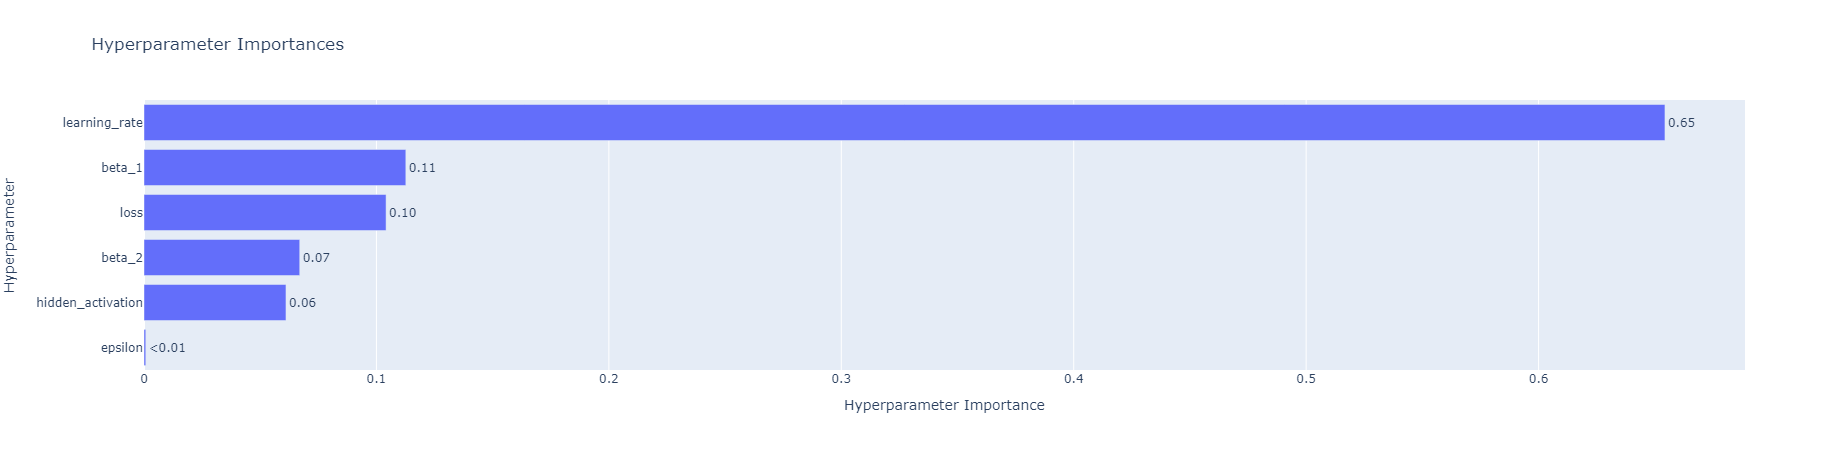
\includegraphics[width=1\columnwidth]{F Nadam Hyp Opt Res Imp.png}}
\caption{Nadam Final Hyperparameter Tuning, parameter Importance}
\label{fig:F Nadam Hyp Opt Res Imp}
\end{figure}

\FloatBarrier

\begin{table}[htbp]
    \centering
    \begin{tabular}{|r|c|c|}\hline
 Parameter& Tuned Value&Importance\\\hline
        \hline
        hidden\_activation& tanh&0.06\\ \hline
        beta\_1& 0.9254&0.11\\ \hline
        beta\_2& 0.9424&0.07\\ \hline
        epsilon& 9.2436e-8&0.005\\ \hline
         learning\_rate& 1.0587e-3&0.65\\ \hline
        loss function & categorical\_crossentropy&0.1\\\hline
    \end{tabular}
    \caption{Nadam Parameter Tuning Result}
    \label{tab:NadamFinalParams}
\end{table}

\FloatBarrier

\begin{figure}[htbp]
\centerline{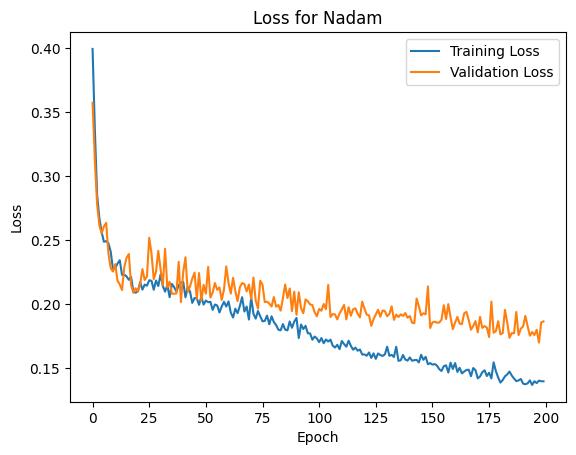
\includegraphics[width=0.9\columnwidth]{F Nadam Loss Graph.png}}
\caption{Nadam Best Model Validation Loss and Loss}
\label{fig:F Nadam Loss Graph}
\end{figure}

\FloatBarrier

The model has some overfitting, but it is not significant. The model is able to generalise the test data well.
The learning rate has a significant effect on the model's performance.
Beta 1, Beta 2, loss function and hidden layer activation function moderately affect the model's performance. ``Fig.~\ref{fig:F Nadam Hyp Opt Res Imp}''
Epsilon has very little effect on the model's performance. \cite{b2}

\newpage

\subsection{Final Testing Results All}

\begin{figure}[htbp]
\centerline{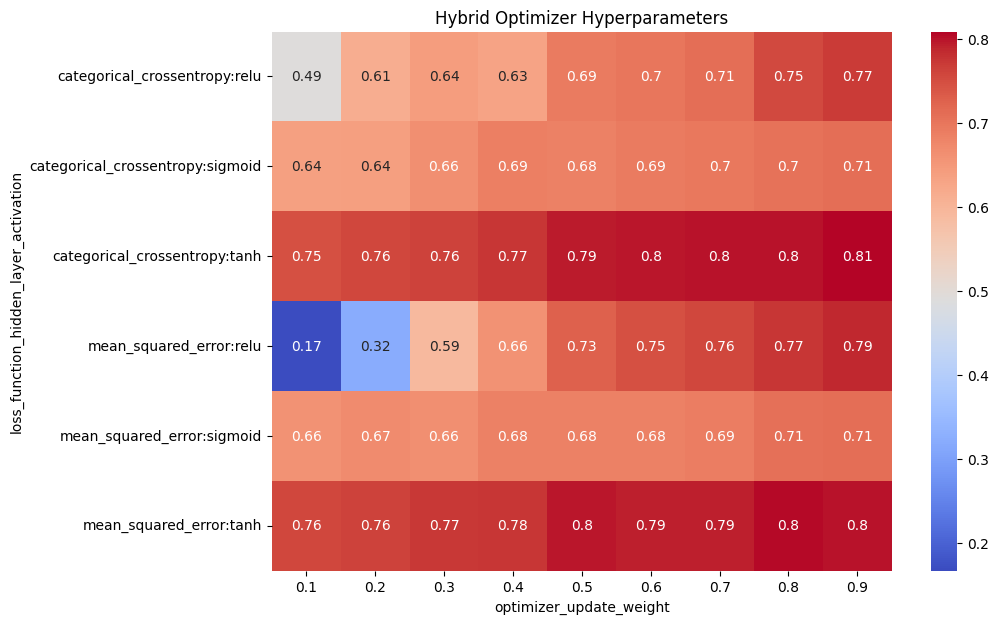
\includegraphics[width=0.9\columnwidth]{F HO GS HM ouw loss ha.png}}
\caption{Heatmap for the Hybrid Optimisation algo. over 165 epochs.}
\label{fig:F HO GS HM ouw loss ha}
\end{figure}

% \newpage
\FloatBarrier

\begin{figure}[htbp]
\centerline{\includegraphics[width=0.9\columnwidth]{F HO loss graph.png}}
\caption{Hybrid Optimisation algo. over 165 epochs. Best Model Validation Loss and Loss}
\label{fig:F HO loss graph}
\end{figure}

\FloatBarrier

\newpage

Grid Search Heat Maps for the three optimizers, using best-tuned hyperparameters, over 50 epochs

\begin{figure}[htbp]
\centerline{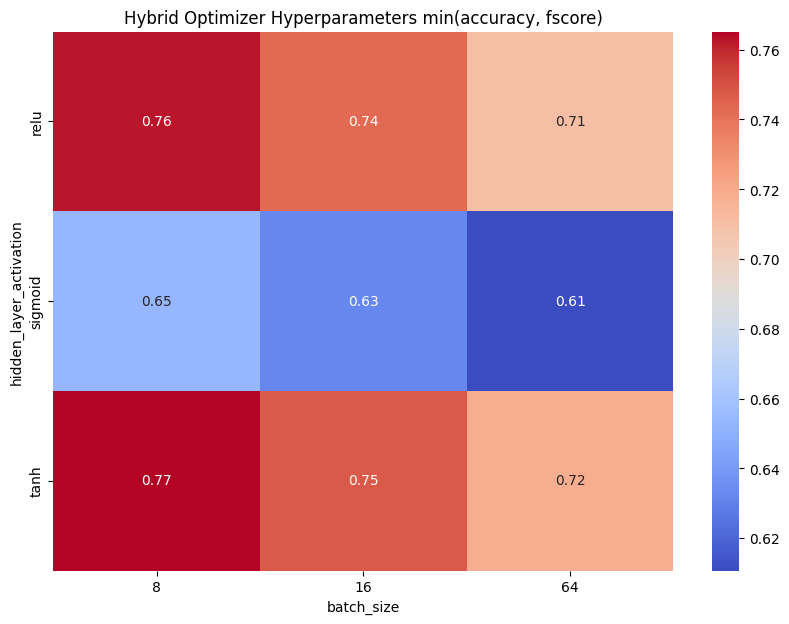
\includegraphics[width=0.8\columnwidth]{Fs HO GS HM acc.png}}
\caption{Hybrid Heatmap}
\label{fig:Fs HO GS HM acc}
\end{figure}

% \newpage
\FloatBarrier

\begin{figure}[htbp]
\centerline{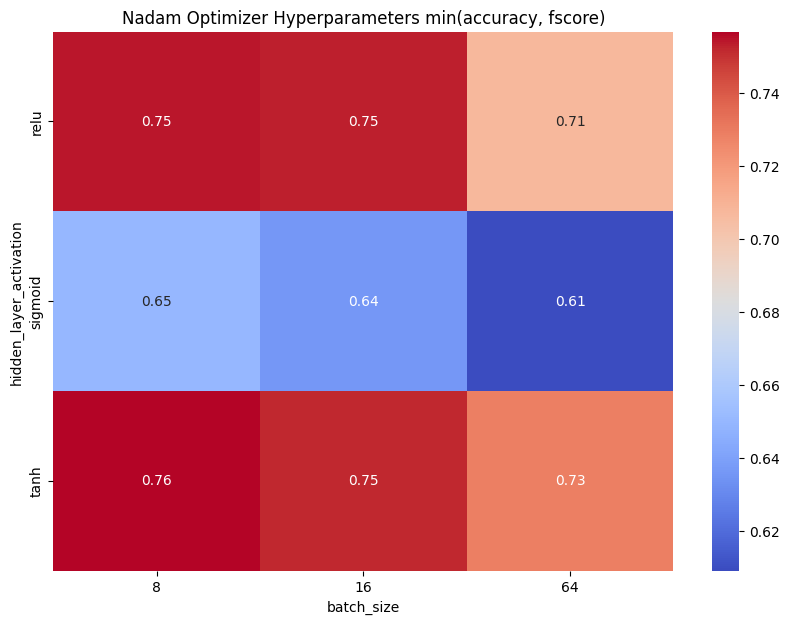
\includegraphics[width=0.8\columnwidth]{Fs Nadam GS HM acc.png}}
\caption{Nadam Heatmap}
\label{fig:Fs Nadam GS HM acc}
\end{figure}

% \newpage
\FloatBarrier

\begin{figure}[htbp]
\centerline{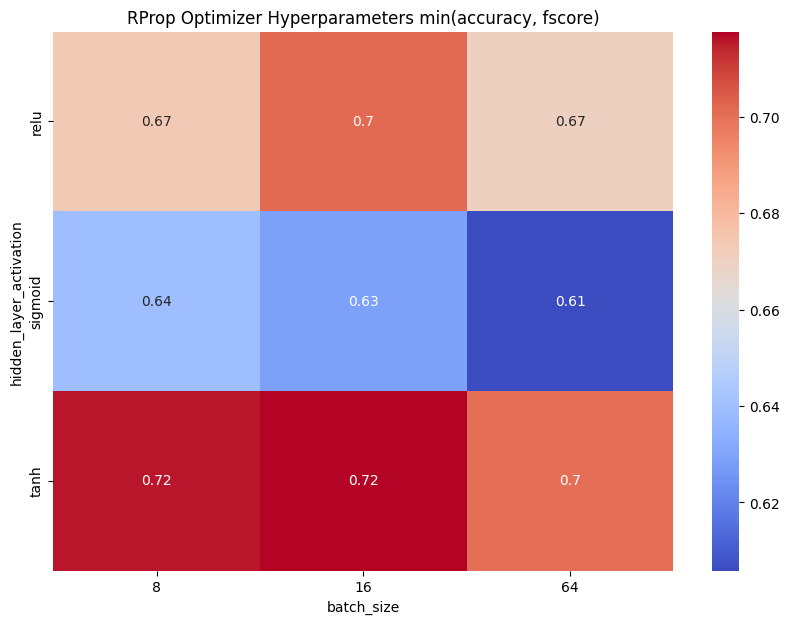
\includegraphics[width=0.8\columnwidth]{Fs RProp GS HM acc.png}}
\caption{RProp Heatmap}
\label{fig:Fs RProp GS HM acc}
\end{figure}

\FloatBarrier

\newpage

Final Results

\begin{table}[!ht]
    \centering
    \begin{tabular}{|l|l|l|l|l|l|} \hline 
    
        & accuracy & fscore & accuracy\_std & fscore\_std & epochs \\ \hline  
        Hybrid & 0.8082 & 0.8089 & 0.0168 & 0.0170 & 165 \\ \hline  
        RProp & 0.7912 & 0.7919 & 0.0031 & 0.0029 & 200 \\ \hline  
        Nadam & 0.8396 & 0.8396 & 0.0057 & 0.0056 & 200 \\ \hline 
    \end{tabular}
    \caption{Final Results: Hybrid, Nadam, RProp}
    \label{tab:FinalResults}
\end{table}

\FloatBarrier

As shown by the heatmap for hybrid optimization ``Fig.~\ref{fig:F HO GS HM ouw loss ha}'', the Nadam optimizer still performs the best and TanH activation function also generally performs the best. This is likely because Nadam is better at managing oscillation than RProp. Additionally, RProp does not necessarily update weights every epoch, meaning it might need many more epochs to train to the same level.

The heatmaps for the 50-epoch models show that the hybrid optimization model can perform better than both Nadam and RProp ``Fig.~\ref{fig:Fs HO GS HM acc},~\ref{fig:Fs Nadam GS HM acc},~\ref{fig:Fs RProp GS HM acc}''. This is likely because the hybrid does better before any overfitting even starts to occur. With the experiments run, the point at which overfitting starts to occur is at around 50 epochs on average ``Fig.~\ref{fig:F Nadam Loss Graph}'' (25 for the final Hybrid Optimization ``Fig.~\ref{fig:F HO loss graph}''). This shows that RProp is more susceptible to overfitting. We know this because the final results of this experiment were run at 165 to 200 epochs and still show an increase in accuracy for each learning algorithm by about 4-7\%, with Nadam sowing the best results. However, it is also possible that if the hybrid were to be trained to 200 epochs, it could show better results than Nadam, but it would be overfitting at that point, and it is most likely that the average weighting for the hybrid would still favour Nadam.

\section{Conclusion}

Overall, the hybrid optimization does not perform as well as Nadam. This is likely because the two optimizers' weight update values can point in opposite directions, and with RProp not necessarily updating weights every epoch, which would hinder Nadam.

The theoretically "best" data preprocessing method does not always yield the best results. This can be seen by the fact that the highest observed result was 84.5\% with the original method 1 of preprocessing on Nadam.

\newpage

\begin{thebibliography}{00}
\bibitem{b1} Gómez, I., Franco, L. \& Jerez, J.M. Neural Network Architecture Selection: Can Function Complexity Help?. \textit{Neural Process Lett} \textbf{30}, 71–87 (2009). https://doi-org.uplib.idm.oclc.org/10.1007/s11063-009-9108-2 

\bibitem{b2} Jordaan, D. \textit{Almond-Classification-COS-711-Assignment-2-2024} https://github.com/DamianJordaan/Almond-Classification-COS-711-Assignment-2-2024

\bibitem{b3} Martín Abadi, Ashish Agarwal, Paul Barham, Eugene Brevdo,
Zhifeng Chen, Craig Citro, Greg S. Corrado, Andy Davis,
Jeffrey Dean, Matthieu Devin, Sanjay Ghemawat, Ian Goodfellow,
Andrew Harp, Geoffrey Irving, Michael Isard, Rafal Jozefowicz, Yangqing Jia,
Lukasz Kaiser, Manjunath Kudlur, Josh Levenberg, Dan Mané, Mike Schuster,
Rajat Monga, Sherry Moore, Derek Murray, Chris Olah, Jonathon Shlens,
Benoit Steiner, Ilya Sutskever, Kunal Talwar, Paul Tucker,
Vincent Vanhoucke, Vijay Vasudevan, Fernanda Viégas,
Oriol Vinyals, Pete Warden, Martin Wattenberg, Martin Wicke,
Yuan Yu, and Xiaoqiang Zheng.
\emph{TensorFlow: Large-scale machine learning on heterogeneous systems,
2015.} Software available from tensorflow.org.

\bibitem{b4}
Dami Choi, Christopher J. Shallue, Zachary Nado, Jaehoon Lee, Chris J. Maddison, and George E. Dahl.
\textit{On Empirical Comparisons of Optimizers for Deep Learning}.
arXiv preprint arXiv:1910.05446v3, 2020. Available at: 
https://arxiv.org/pdf/1910.05446

\bibitem{b5}
Robin M. Schmidt, Frank Schneider, and Philipp Hennig.
\textit{Descending through a Crowded Valley — Benchmarking Deep Learning Optimizers}.
arXiv preprint arXiv:2007.01547v6, 2021. Available at: https://arxiv.org/pdf/2007.01547

\end{thebibliography}

\end{document}
